% Options for packages loaded elsewhere
\PassOptionsToPackage{unicode}{hyperref}
\PassOptionsToPackage{hyphens}{url}
%
\documentclass[
]{book}
\usepackage{lmodern}
\usepackage{amssymb,amsmath}
\usepackage{ifxetex,ifluatex}
\ifnum 0\ifxetex 1\fi\ifluatex 1\fi=0 % if pdftex
  \usepackage[T1]{fontenc}
  \usepackage[utf8]{inputenc}
  \usepackage{textcomp} % provide euro and other symbols
\else % if luatex or xetex
  \usepackage{unicode-math}
  \defaultfontfeatures{Scale=MatchLowercase}
  \defaultfontfeatures[\rmfamily]{Ligatures=TeX,Scale=1}
\fi
% Use upquote if available, for straight quotes in verbatim environments
\IfFileExists{upquote.sty}{\usepackage{upquote}}{}
\IfFileExists{microtype.sty}{% use microtype if available
  \usepackage[]{microtype}
  \UseMicrotypeSet[protrusion]{basicmath} % disable protrusion for tt fonts
}{}
\makeatletter
\@ifundefined{KOMAClassName}{% if non-KOMA class
  \IfFileExists{parskip.sty}{%
    \usepackage{parskip}
  }{% else
    \setlength{\parindent}{0pt}
    \setlength{\parskip}{6pt plus 2pt minus 1pt}}
}{% if KOMA class
  \KOMAoptions{parskip=half}}
\makeatother
\usepackage{xcolor}
\IfFileExists{xurl.sty}{\usepackage{xurl}}{} % add URL line breaks if available
\IfFileExists{bookmark.sty}{\usepackage{bookmark}}{\usepackage{hyperref}}
\hypersetup{
  pdftitle={Data Management SOP for the Tampa Bay Estuary Program},
  pdfauthor={Marcus W. Beck},
  hidelinks,
  pdfcreator={LaTeX via pandoc}}
\urlstyle{same} % disable monospaced font for URLs
\usepackage{longtable,booktabs}
% Correct order of tables after \paragraph or \subparagraph
\usepackage{etoolbox}
\makeatletter
\patchcmd\longtable{\par}{\if@noskipsec\mbox{}\fi\par}{}{}
\makeatother
% Allow footnotes in longtable head/foot
\IfFileExists{footnotehyper.sty}{\usepackage{footnotehyper}}{\usepackage{footnote}}
\makesavenoteenv{longtable}
\usepackage{graphicx,grffile}
\makeatletter
\def\maxwidth{\ifdim\Gin@nat@width>\linewidth\linewidth\else\Gin@nat@width\fi}
\def\maxheight{\ifdim\Gin@nat@height>\textheight\textheight\else\Gin@nat@height\fi}
\makeatother
% Scale images if necessary, so that they will not overflow the page
% margins by default, and it is still possible to overwrite the defaults
% using explicit options in \includegraphics[width, height, ...]{}
\setkeys{Gin}{width=\maxwidth,height=\maxheight,keepaspectratio}
% Set default figure placement to htbp
\makeatletter
\def\fps@figure{htbp}
\makeatother
\setlength{\emergencystretch}{3em} % prevent overfull lines
\providecommand{\tightlist}{%
  \setlength{\itemsep}{0pt}\setlength{\parskip}{0pt}}
\setcounter{secnumdepth}{5}
\usepackage{booktabs}
\usepackage{amsthm}
\makeatletter
\def\thm@space@setup{%
  \thm@preskip=8pt plus 2pt minus 4pt
  \thm@postskip=\thm@preskip
}
\makeatother
\usepackage[]{natbib}
\bibliographystyle{apalike}

\title{Data Management SOP for the Tampa Bay Estuary Program}
\author{Marcus W. Beck}
\date{2021-01-07}

\begin{document}
\maketitle

{
\setcounter{tocdepth}{1}
\tableofcontents
}
\hypertarget{prerequisites}{%
\chapter{Prerequisites}\label{prerequisites}}

\hypertarget{background}{%
\chapter{Background}\label{background}}

\hypertarget{importance-of-data}{%
\section{Importance of data}\label{importance-of-data}}

\begin{itemize}
\tightlist
\item
  Data are the foundation of all research products and management decisions
\item
  A data definition, e.g., raw information in flat files, synthesized/derived datasets, models, etc.
\item
  How data are used in applied research/environmental sciences
\end{itemize}

\hypertarget{why-we-need-to-effectively-manage-data}{%
\section{Why we need to effectively manage data}\label{why-we-need-to-effectively-manage-data}}

\begin{itemize}
\tightlist
\item
  What happens when data are not managed properly - Figure 1, bit-rot
\item
  Professorware
\item
  Benefits of a data management workflow
\item
  Applications in open science
\end{itemize}

\hypertarget{goalsobjectives-of-this-document}{%
\section{Goals/objectives of this document}\label{goalsobjectives-of-this-document}}

\begin{itemize}
\tightlist
\item
  What it is, what it is not - including what makes TBEP different from other organizations, i.e., we have hands in lots of projects vs one central product (e.g., OHI), so our SOP needs to be generalizable
\item
  Develop pathway for metadata
\item
  Intended audience
\end{itemize}

\begin{figure}
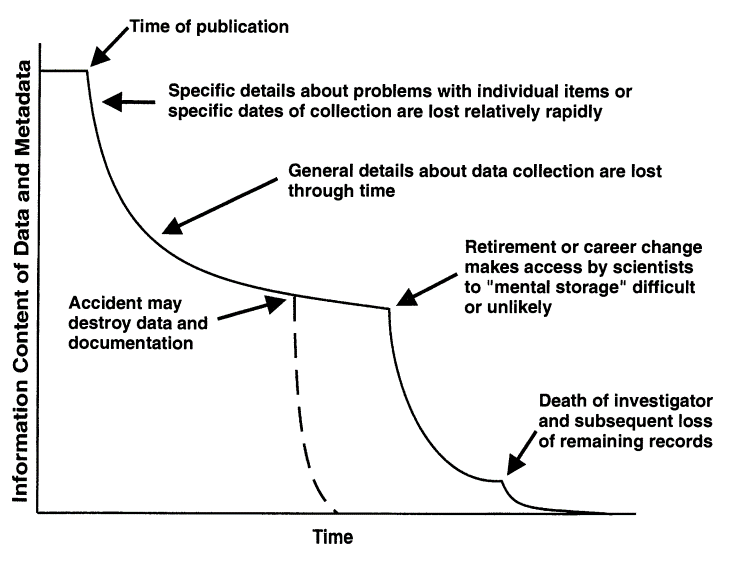
\includegraphics[width=10.19in]{img/michener} \caption{Loss of information over time in the absence of data management [@Michener97]}\label{fig:michener}
\end{figure}

\hypertarget{keys}{%
\chapter{Key Concepts and Principles}\label{keys}}

\hypertarget{general-concepts}{%
\section{General concepts}\label{general-concepts}}

\begin{itemize}
\tightlist
\item
  What are data, i.e., from the perspective of the researcher/agency scientist/manager?

  \begin{itemize}
  \tightlist
  \item
    Workflow (e..g, operationalizing Twitter scraping), dataset (field/lab data), model products, etc.
  \item
    Ask yourself, who is going to use this and how do I make their lives ``easier'' by opening the data using FAIR principles?
  \end{itemize}
\item
  The FAIR principles (very broad, emphasize throughout), also general open science definition and how data relates to open science (channel PeerJ paper distinction)
\end{itemize}

\hypertarget{specific-concepts}{%
\section{Specific concepts}\label{specific-concepts}}

\begin{itemize}
\tightlist
\item
  Specific concepts (particularly for tabular data)

  \begin{itemize}
  \tightlist
  \item
    an overview of tidy data, can a machine read it?
  \item
    normalized tables (including discussion of key variables), what are unique ids (e.g., tberf oyster, how did I make the unique id?), facilitate standard DB queries
  \item
    metadata documentation (min requirements, relevant standards)
  \end{itemize}
\item
  types of data products (e.g., raw data, models, synthesized/derived data, etc.) or types of data (flat file, spatial, disparate)
\item
  how-to cookbooks for data prep (could speak to different parts of the analysis workflow, e.g., project inception, mid-project, post-project/damage control) for archival, naming conventions (e.g., no spaces, short but descriptive, etc.), data dictionaries
\item
  where do data live long-term, what's a doi, considering a data paper, federated repository, etc.

  \begin{itemize}
  \tightlist
  \item
    GitHub repository
  \item
    Stable URL
  \item
    Official repository
  \end{itemize}
\end{itemize}

\hypertarget{workflow}{%
\chapter{Data Management Workflow}\label{workflow}}

\begin{itemize}
\tightlist
\item
  Setup some kind of flow chart (if this, then that)

  \begin{itemize}
  \tightlist
  \item
    What type of project am I working on?
  \item
    What types of products am I expecting?
  \item
    Where am I at with the project (beginning, middle, end/damage control)?
  \item
    How do I want to make the data accessible?
  \end{itemize}
\end{itemize}

\hypertarget{cases}{%
\chapter{Case Studies}\label{cases}}

Demonstrate the workflow

\hypertarget{tberf-oyster-restoration-project}{%
\section{TBERF oyster restoration project}\label{tberf-oyster-restoration-project}}

\hypertarget{desotorestore-project}{%
\section{DeSoto/RESTORE project}\label{desotorestore-project}}

\hypertarget{red-tide-twitter-repo}{%
\section{Red Tide Twitter repo}\label{red-tide-twitter-repo}}

\hypertarget{final}{%
\chapter{Final Words}\label{final}}

\begin{itemize}
\tightlist
\item
  emphasis on ``something is better than nothing'', fully open is ideal but difficult to achieve
\item
  Just remember FAIR
\end{itemize}

\hypertarget{appendices}{%
\chapter{Appendice}\label{appendices}}

\hypertarget{guidelines-for-best-data-management-practices}{%
\section{Guidelines for best data management practices}\label{guidelines-for-best-data-management-practices}}

\hypertarget{data-types}{%
\section{Data types}\label{data-types}}

\begin{itemize}
\tightlist
\item
  Field data

  \begin{itemize}
  \tightlist
  \item
    Survey forms
  \item
    Tabular*
  \item
    Database of tables
  \end{itemize}
\item
  Database

  \begin{itemize}
  \tightlist
  \item
    Synthesis
  \item
    New
  \end{itemize}
\item
  Model

  \begin{itemize}
  \tightlist
  \item
    Actual model
  \item
    Model results
  \end{itemize}
\item
  Dashboard
\end{itemize}

\hypertarget{definitions}{%
\section{Definitions}\label{definitions}}

Dashboard
Data
Aggregation vs.~synthesis
Model
Tabular
Database
Flat file
Tidy data

\hypertarget{metadata-templates}{%
\section{Metadata templates}\label{metadata-templates}}

General - Who, what, when, where, why?

Specific - XML, EML, etc.

  \bibliography{refs.bib}

\end{document}
